\documentclass[11pt,a4paper,twoside]{article}
\usepackage{geometry}
\geometry{a4paper, margin=2cm}
\usepackage{graphicx}
\usepackage{hyperref}

\begin{document}
\begin{center}
    \Large{\textbf{IDP Software documentation}}
    
    \Large{Team M208}
\end{center}
\vspace{0.05cm}

\section{Introduction}

In the Integrated Design Project, a robot must be built which can pick up cubes and sort them. For this task,
an algorithm dictating how the robot moves on the board was developed. 
The code can be found on GitHub: \url{https://github.com/gca30/IDP/blob/main/Software/sketch_nov06a/sketch_nov06a.ino}


\section{Main structure}

\begin{center}
    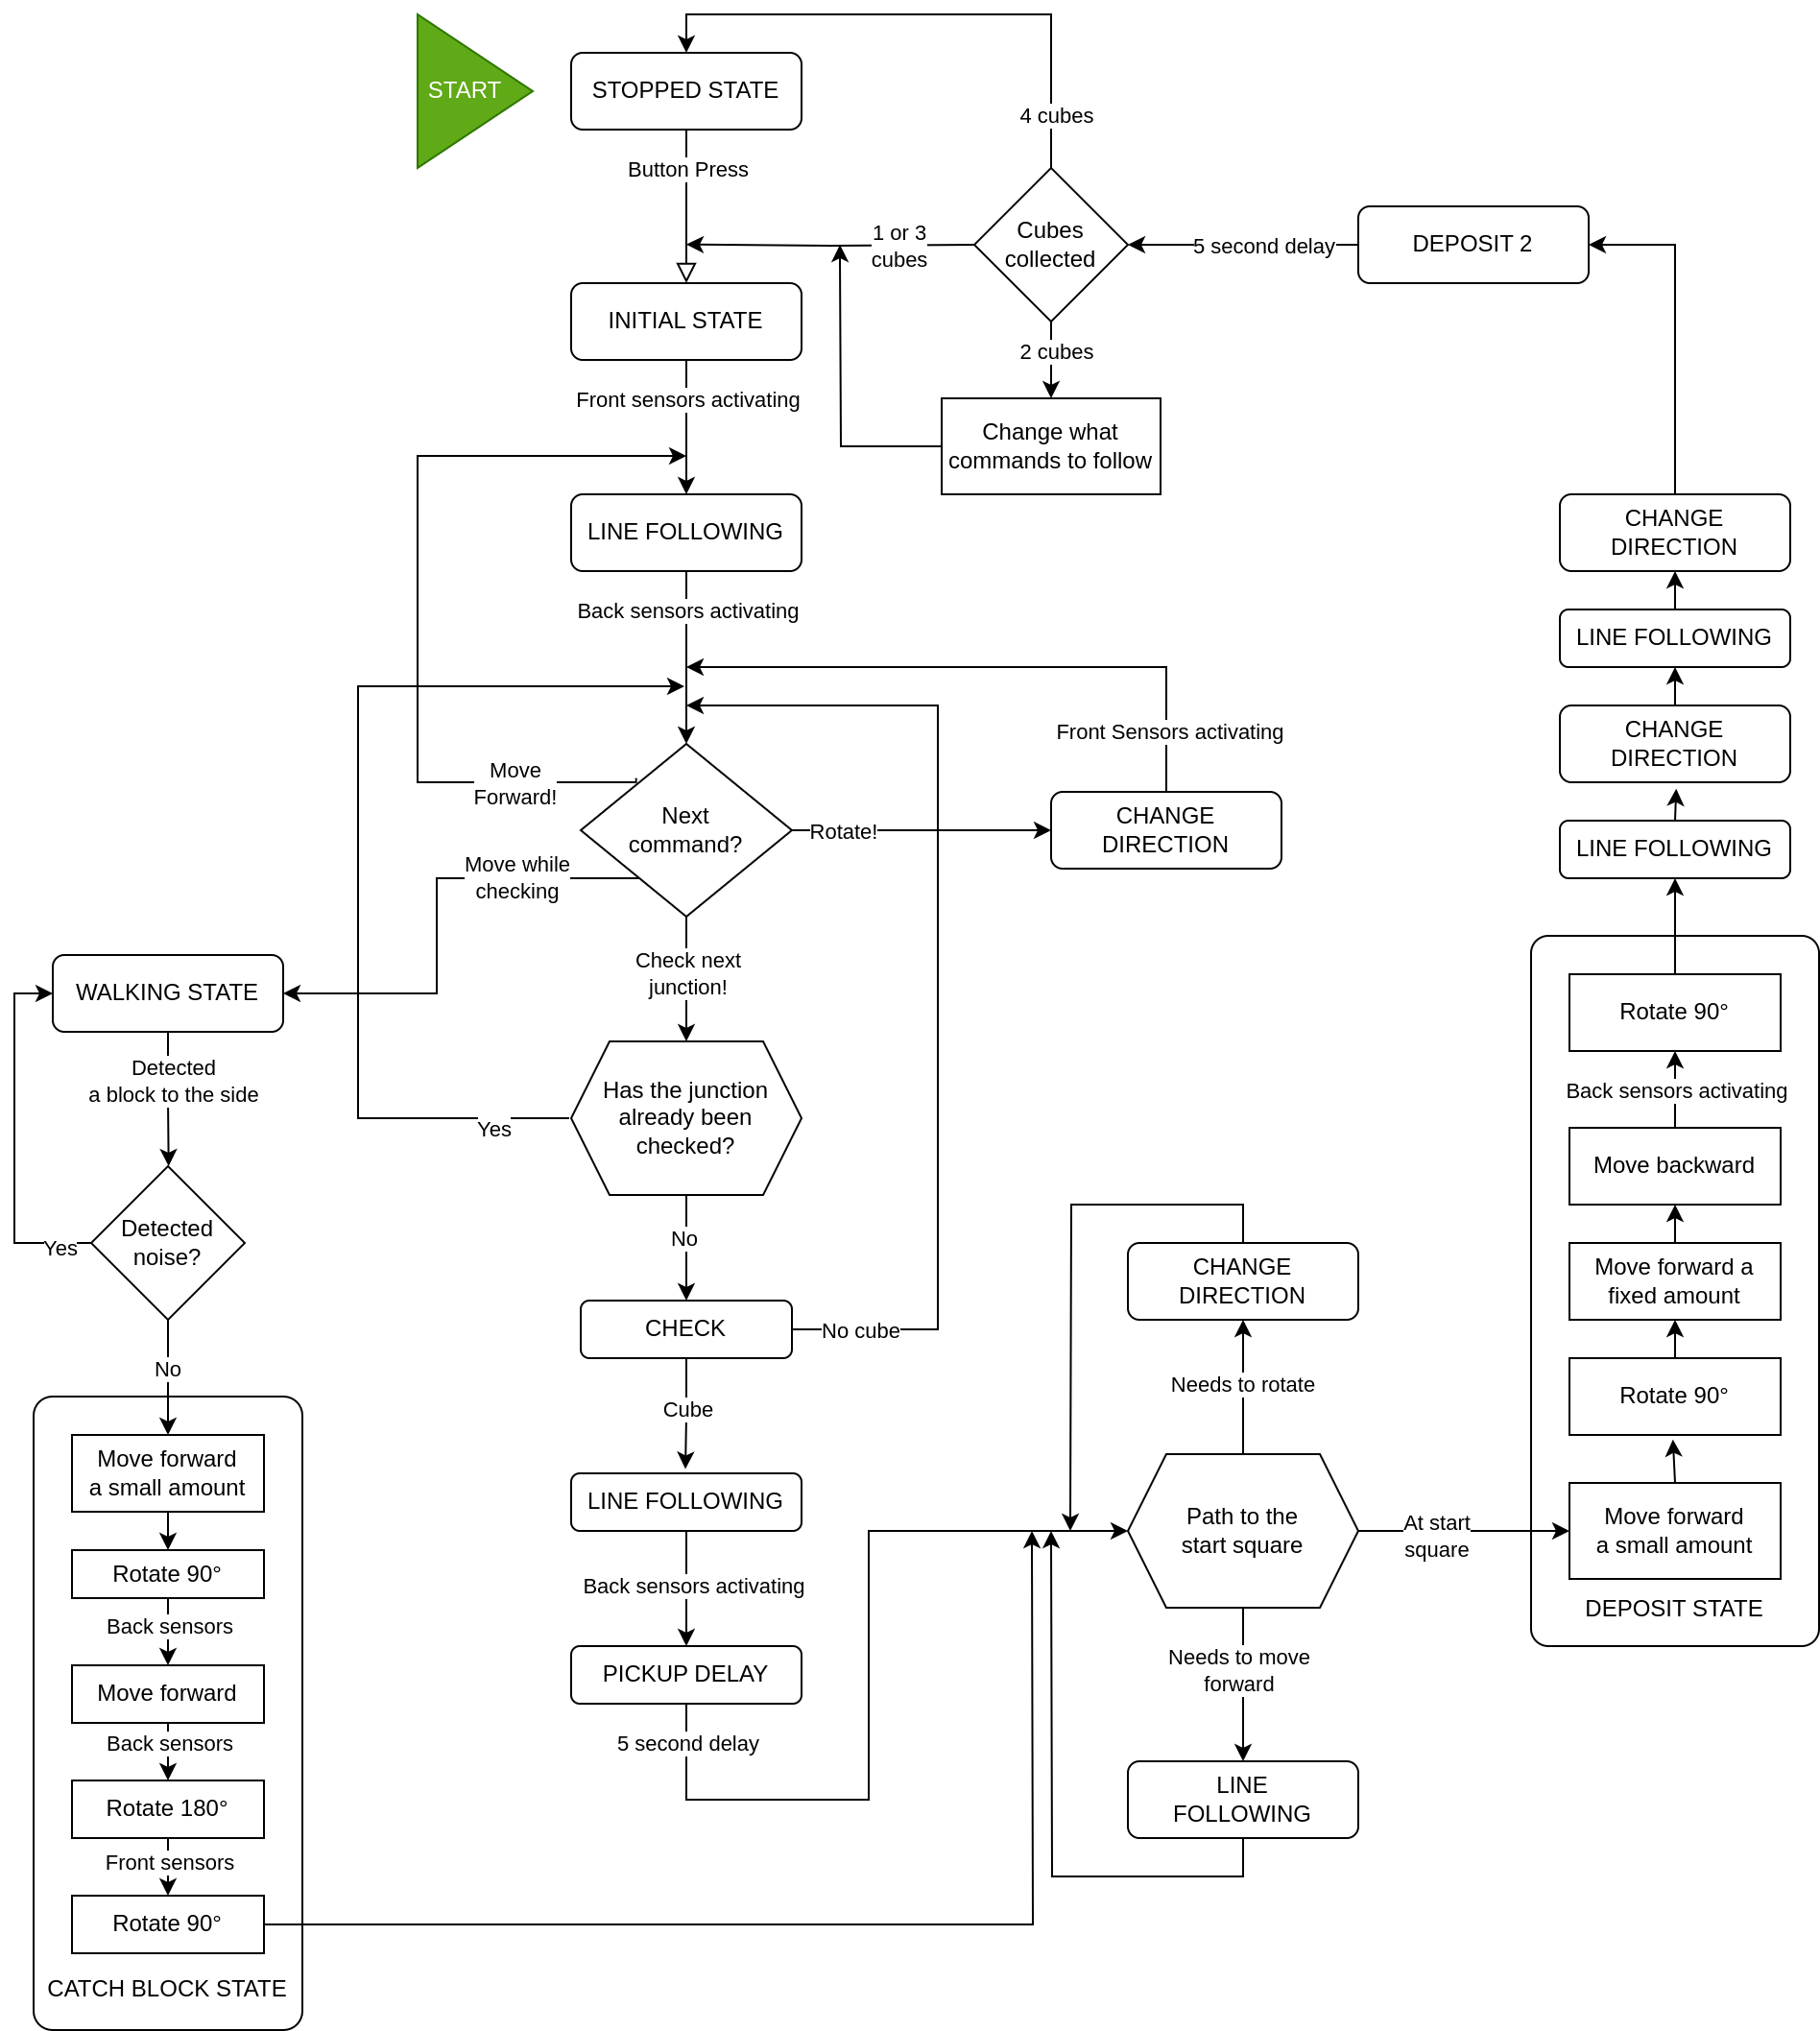
\includegraphics[width=0.8\textwidth]{flowchart}
\end{center}

The whole algorithm is detailed in the above flowchart. The program running on the micro-controller
is always in a specific \textbf{state}. Each state has a unique loop functions, which
runs repeatedly on an interval, and a startup function, that runs when the program switches to that state.
The values read from the sensors are able to change the states, and
states dictate how the robot moves.

In the standard Arduino \verb|startup| function, all the sensors and motors are
initialized. In the standard \verb|loop| function, all the values of the sensors are read.
Some more logic is ran in the \verb|stateSensors| function, after which the 
specific loop function is ran. The state setup functions are ran in the \verb|setState| function.

In the flowchart, rounded rectangles are states and rhombuses and hexagons
represents logic, mostly placed in the \verb|switchState| function.
This function uses all the available variables to determine which state to
run next.

Before detecting a cube, it runs a predetermined path, which is
stored as an array of characters called \verb|commands|, of the form: \verb|mcWcmcNcmWcEmcmcScmEc|. 
Each character represents which state to run next, with \verb|c| representing a cube check, 
\verb|m| representing a line following state, while the others represent in which direction to turn.

\section{Variables}

The program keeps as variables the position and orientation of the robot,
how many cubes it has picked up (\verb|TaskState|), what type of cube does it have 
(\verb|CubeState|) and if the blue LED needs to be blinking (\verb|BlueLEDState|).

The position is stored as a number between -3 and 19, such that the positions from
1 to 10 represent the 10 central junctions. The directions were given the values of -5 for North,
-1 for West, 1 for East and 5 for South, as viewed from above. This way, the position can
be updated using a statement of the form \verb|position += direction|.

\section{Input and output}

Movement is done by using the \verb|setMovmenent| function, which switches
the motors to a specific mode: stopping, moving forwards or backwards, 
rotating to the left or to the right, pivoting around a certain wheel, etc.
This made switching from the cardboard prototype to the final chassis easier: even 
if during the placement of the motors, they were switched or inverted, the code
would not drastically need to be changed.

The readings of the ultrasonic and Time Of Flight sensors are the two readings that
need to be taken over a longer period of time to avoid spikes and to increase
accuracy. This is done in the \verb|readUltrasonic| and \verb|time_of_flight| functions.
Each function has an associated array of previous values. Every time the function is called,
it reads a new value, shifting all the previous values by one and placing the new value at the end.
These values are copied into a new array, which is sorted using insertion sort. After this,
the median is returned.

\section{Line following and rotating}

The line following algorithm uses the two line detecting sensors at the front for adjusting its position.
Every loop, it checks whether it is both sensors are high. If one of them is low, then it
rotates opposite to the direction it has rotated in, otherwise it moves forward. One of the conditions for exiting the state is when either of the back sensors are high.
However, the line following state might activate when the robot is already inside a junction, having the back sensors high. The other condition is that the robot has
exited the junction and has had both of its back sensors low before.

The rotate state uses a similar condition, except it rotates until the two front sensors are high and they were both low at some point during the state.
The state takes a parameter, the desired direction the car should be at the end of the state (\verb|desiredDir| variable).
The added complexity of this state is deciding in which direction to rotate. To rotate from West to East, for example, the state might need to be run twice (\verb|rotationIterations| variable), and depending on the position, by turning either left or right. In addition,
some junctions on the edges of the board do not have the grid lines painted in certain directions. The algorithm never chooses these directions.

\end{document}
